\documentclass[17pt,letterpaper]{extarticle}
\usepackage{pdfpages}
\usepackage[utf8]{inputenc}
\usepackage{tocloft}
\usepackage{graphicx}
\usepackage{float}
\usepackage{tikz}
\usepackage{epstopdf}

\newcommand*\circled[1]{\tikz[baseline=(char.base)]{
            \node[shape=circle,draw,inner sep=2pt] (char) {#1};}}

\setlength{\footskip}{100pt}
\renewcommand{\cftsecleader}{\cftdotfill{\cftdotsep}}
\renewcommand{\contentsname}{Table des matières}
\setlength{\parindent}{0ex}

\makeatletter

\def\clearleftpage{\clearpage\ifodd\c@page\else
\hbox{}\newpage\if@twocolumn\hbox{}\newpage\fi\fi}

\makeatother

\title{12 Partitions pour Xylophone \& Métallophone à 8 Barres}
\author{Guilhem Vellut}
\date{}

\begin{document}
\pagestyle{empty}
\includepdfset{pagecommand=\thispagestyle{plain}}
\setcounter{secnumdepth}{-1}
\setcounter{page}{1}

\maketitle
\thispagestyle{empty}

\clearpage
\vspace*{\fill}

{\tiny 1\textsuperscript{ère} édition - Janvier 2018 \\ Mis en page avec LilyPond et \LaTeX \\
Logo de couverture par Freepik de FlatIcon.com\\
\newline
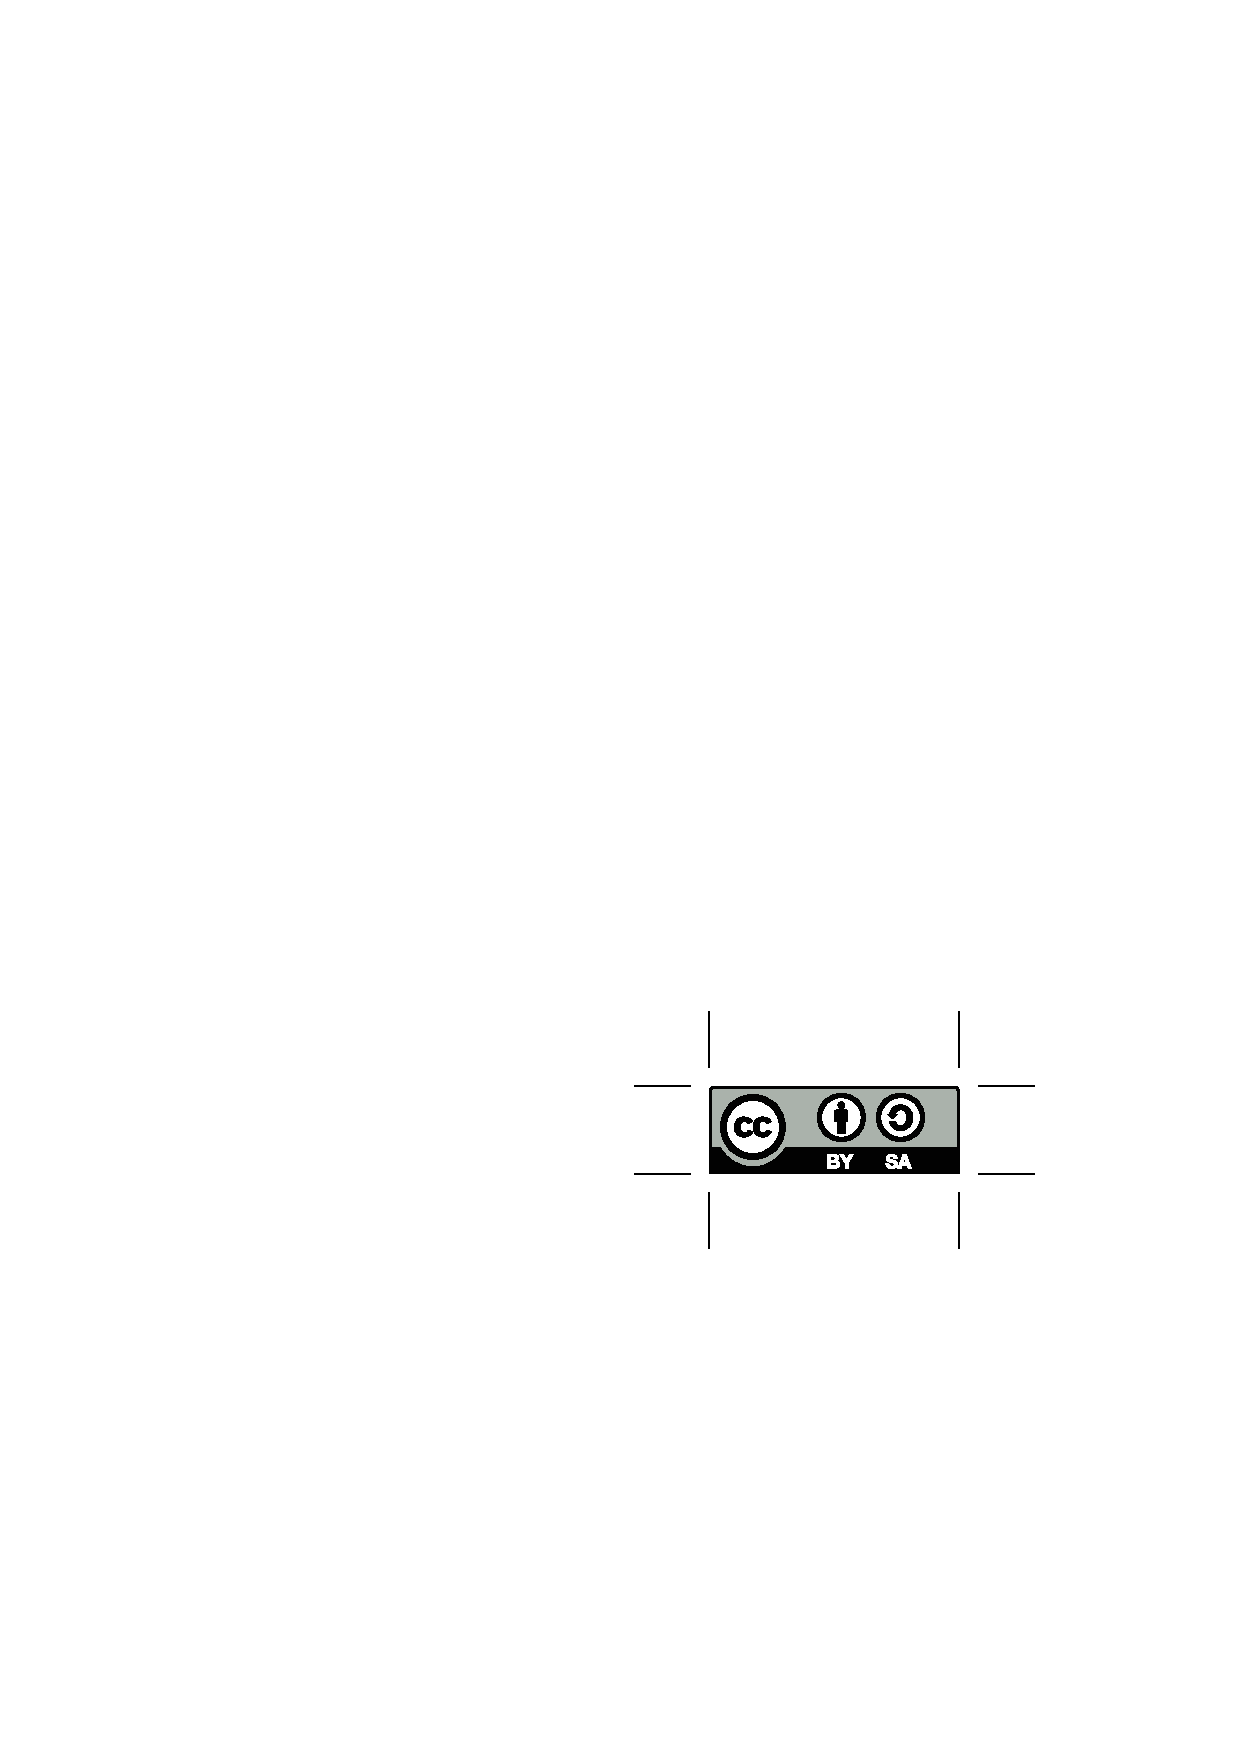
\includegraphics{by-sa} \\
\newline
Partitions CC-BY-SA Guilhem Vellut\\
Contient des partitions adaptées de Jean-Michel Thiémonge / Piano GNU (CC-BY)\\
Contient des partitions adaptées du projet Wikisource Partitions (CC-BY-SA)\\
Voir goo.gl/oMiAjK pour les détails \par}

\clearpage

\tableofcontents
\thispagestyle{empty}

\clearleftpage
\pagestyle{plain} 

\section{Introduction \& Coloriage des notes}

Ce livre contient des partitions pour xylophones et métallophones à 8 barres (1 octave). Elles sont adaptées à la plupart des instruments de ce type vendus pour les enfants, par exemple le Métallophone Animambo ou le Xylophone Fisher-Price.\\

Comme ces partitions sont destinées à des jeunes enfants, j'ai ajouté en-dessous de chaque note une indication de la couleur de la barre du xylophone à taper. Il est ainsi possible de jouer les partitions sans avoir besoin de savoir lire la notation musicale classique.\\

Par contre, ce livre est imprimé en noir et blanc et les couleurs des barres varient selon la marque de l'instrument : il faut donc colorier vous-mêmes les notes selon le schéma de couleurs spécifique à votre xylophone ou métallophone.\\

Pour vous aider, regardez la photo d'un xylophone à 8 barres sur la page suivante.\\

Les barres sont numérotées de \circled{1} à \circled{8} :
\begin{itemize}
  \item \circled{1} pour la barre la plus grande (Do grave) 
  \item \circled{8} pour la barre la plus petite (Do aigu)
  \item Entre les deux Do, la taille des barres diminue : Ré \circled{2}, Mi \circled{3}, Fa \circled{4}, Sol \circled{5}, La \circled{6}, Si \circled{7}
\end{itemize}

\begin{figure}[h]
\centering
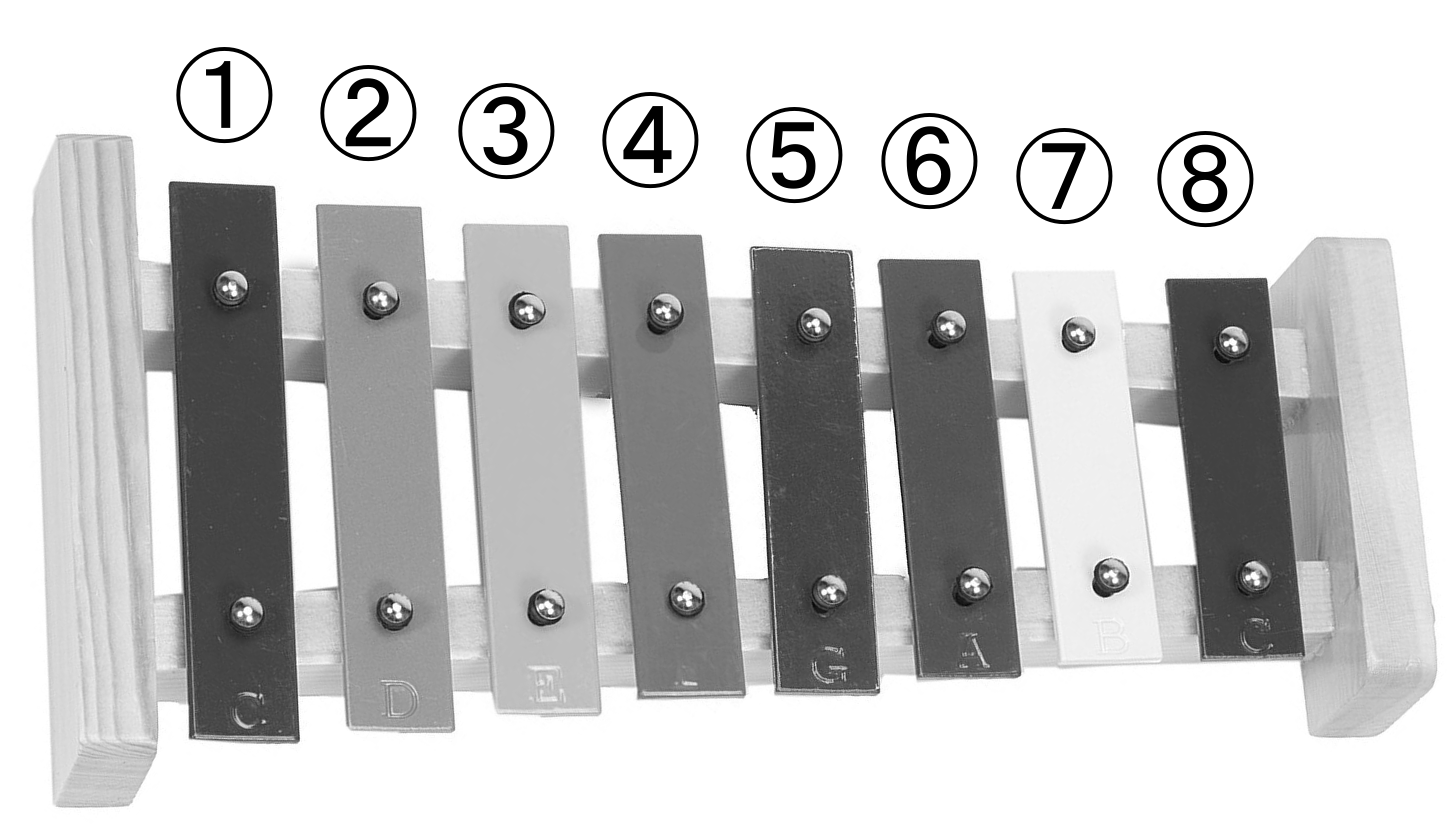
\includegraphics{xylophone_bw.png}
\end{figure}

Toutes les chansons du livre contiennent en entête la liste des barres utilisées dans la partition, de \circled{1} à \circled{8} comme sur la photo. Souvent, toutes les barres de l'instrument ne sont pas utilisées.\\

Pour préparer une partition, il est conseillé de commencer par colorier ces cercles numérotés en utilisant la couleur de la barre correspondante de votre instrument. Ensuite, il faut recopier ces couleurs pour le reste des notes de la partition. Finalement, jouez !

\clearleftpage

\addcontentsline{toc}{section}{Au clair de la Lune}
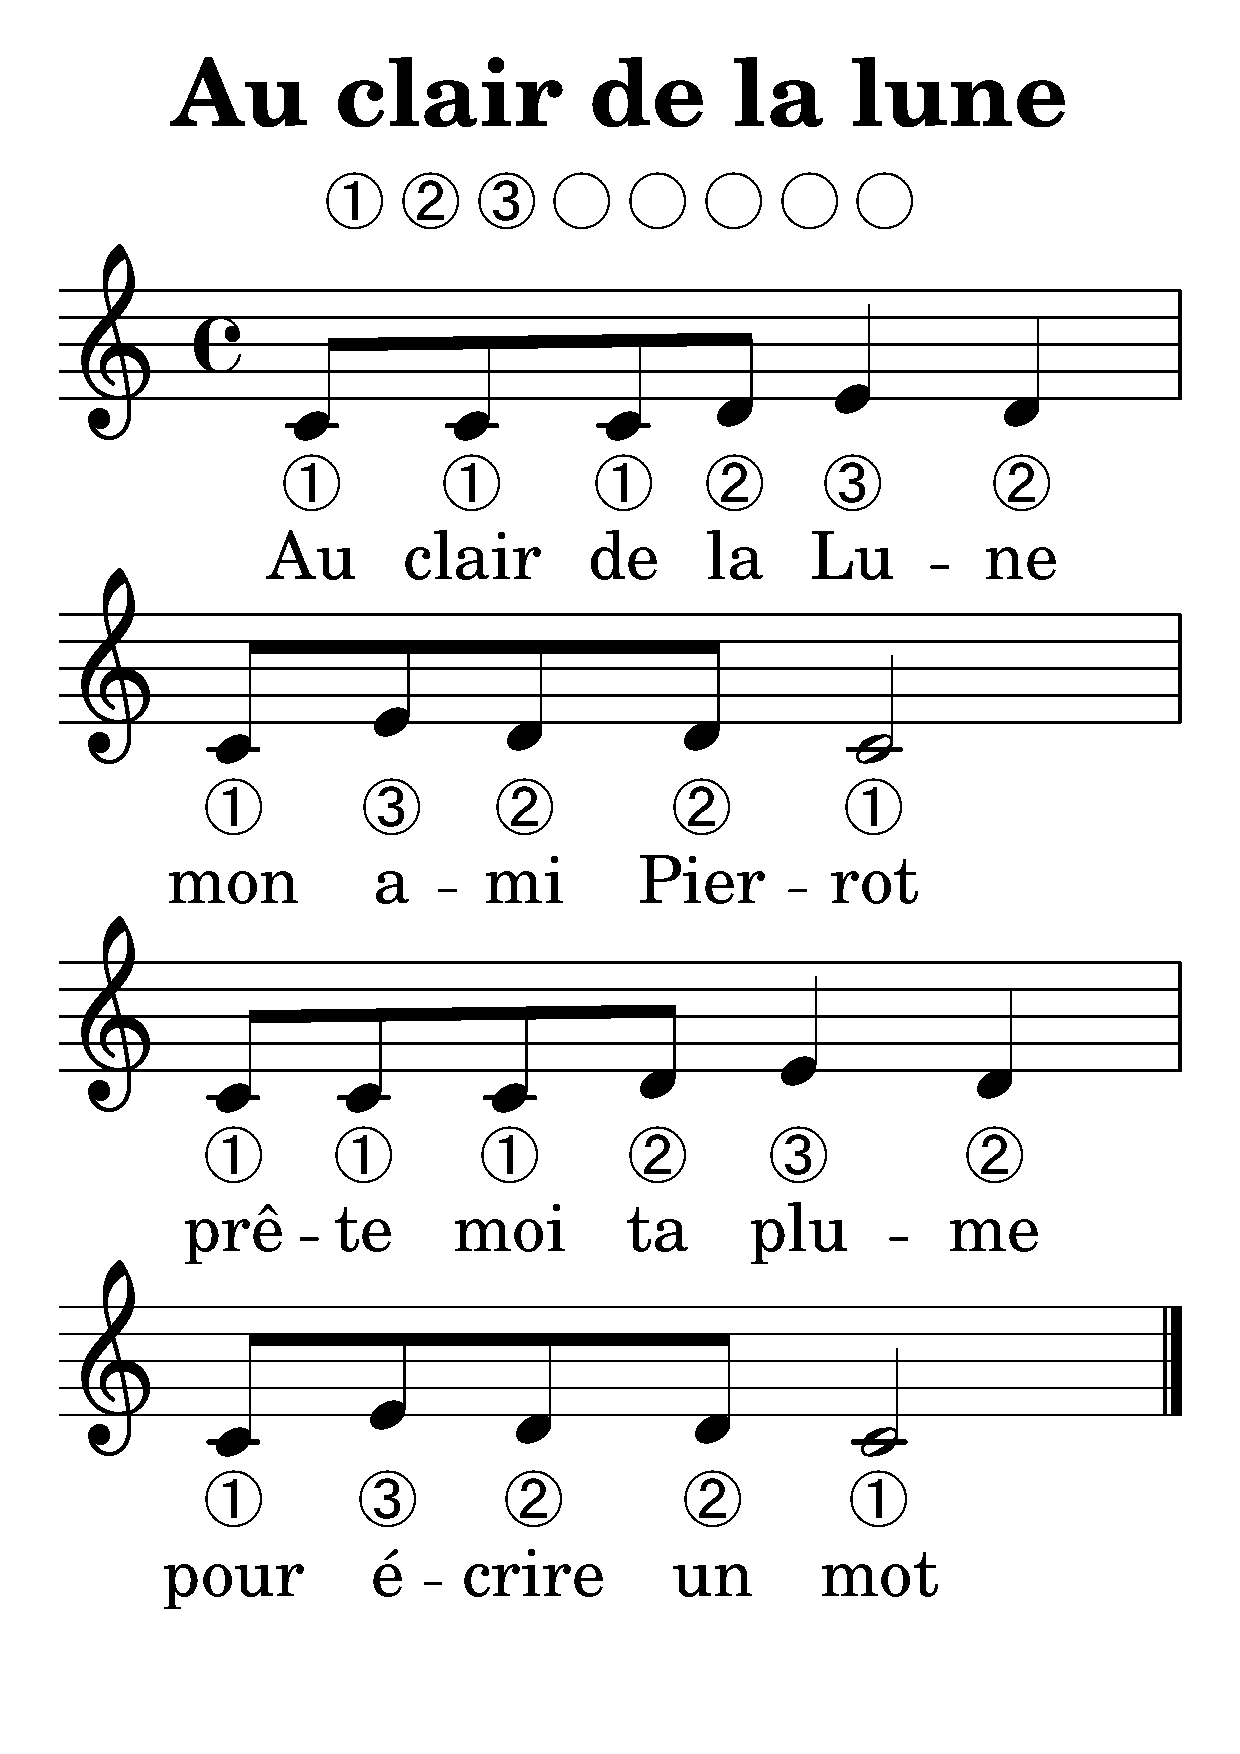
\includepdf[pages=1-,pagecommand={\null\clearpage}]{au_clair_de_la_lune.pdf}

\clearleftpage

\addcontentsline{toc}{section}{L'alphabet}
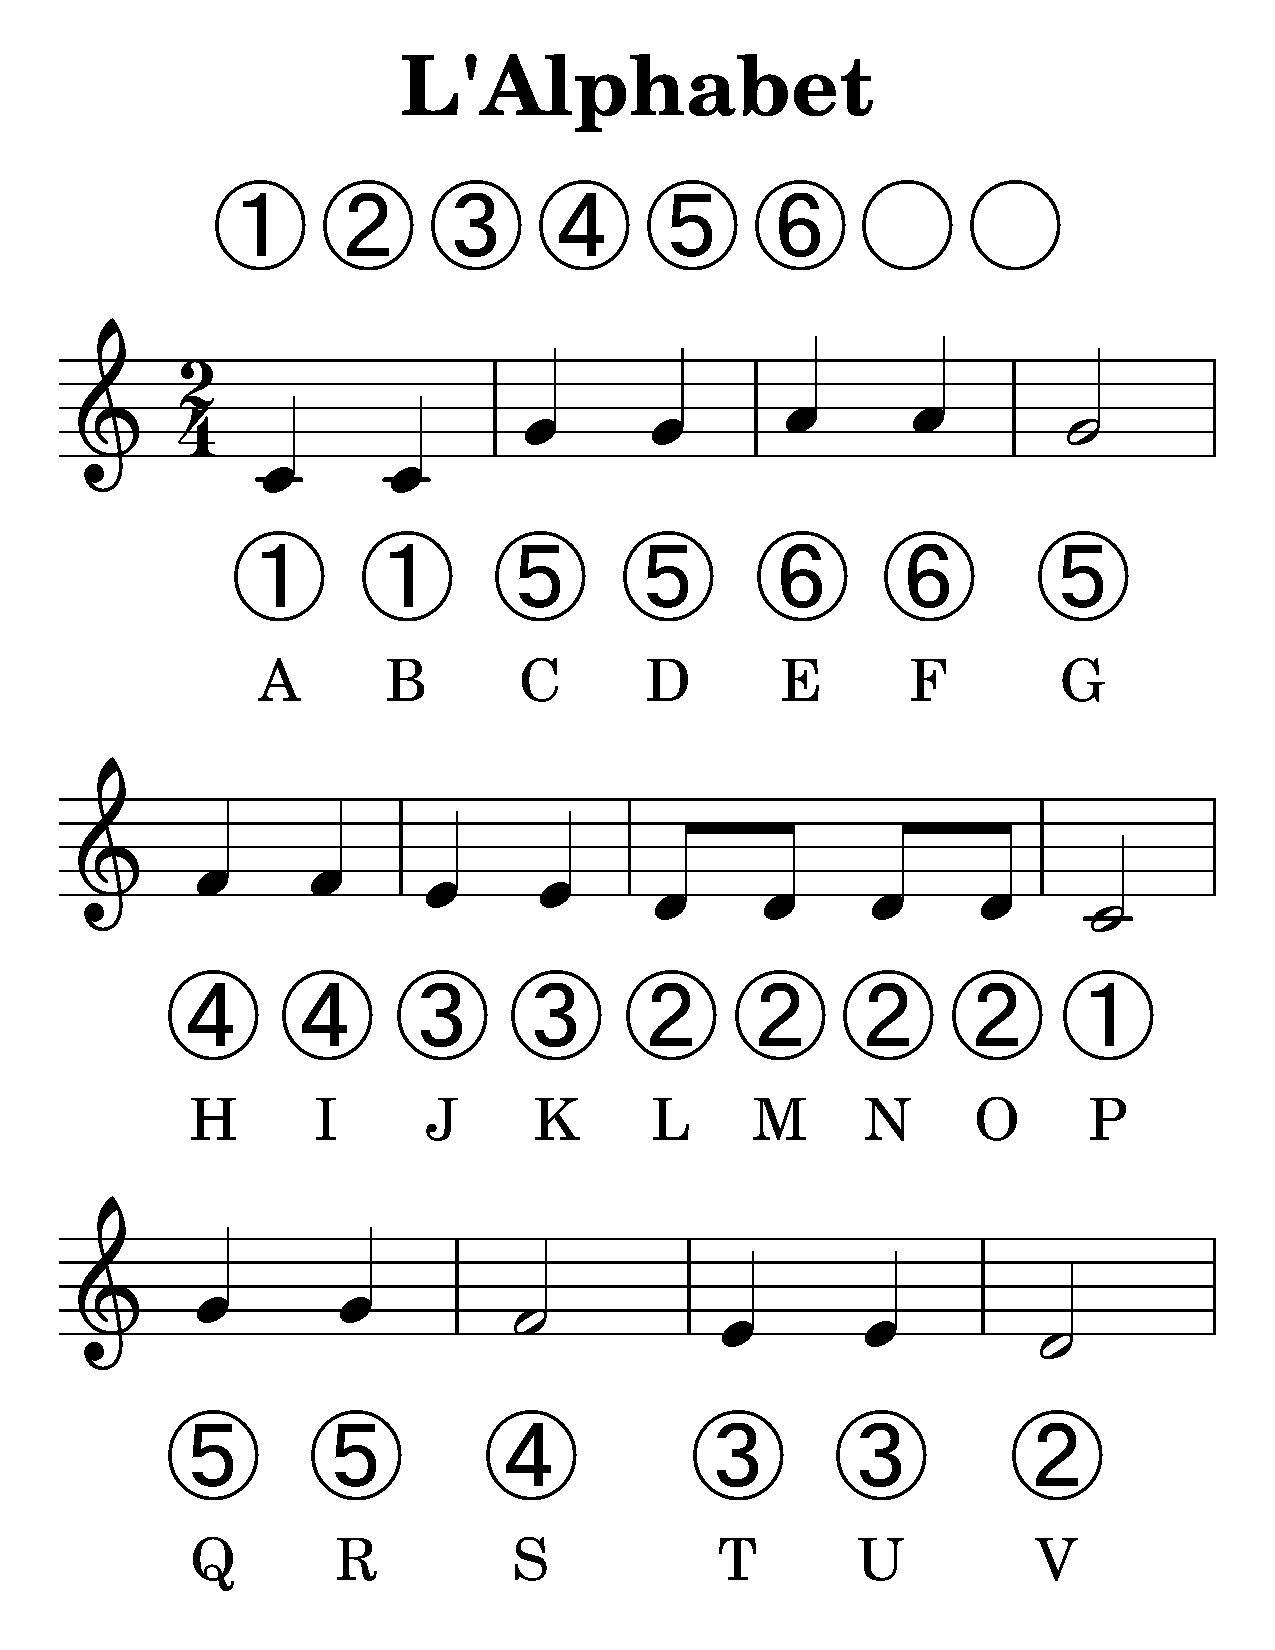
\includepdf[pages=1-,pagecommand={\null\clearpage}]{alphabet_fr.pdf}

\clearleftpage

\addcontentsline{toc}{section}{Pirouette Cacahuète}
\includepdf[pages=1-,pagecommand={\null\clearpage}]{pirouette.pdf}

\clearleftpage

\addcontentsline{toc}{section}{Dansons la capucine}
\includepdf[pages=1-,pagecommand={\null\clearpage}]{dansons_la_capucine.pdf}

\clearleftpage

\addcontentsline{toc}{section}{Il court, il court, le furet}
\includepdf[pages=1-,pagecommand={\null\clearpage}]{furet.pdf}

\clearleftpage

\addcontentsline{toc}{section}{Promenons-nous dans les bois}
\includepdf[pages=1-,pagecommand={\null\clearpage}]{promenons_nous.pdf}

\clearleftpage

\addcontentsline{toc}{section}{Vive le vent}
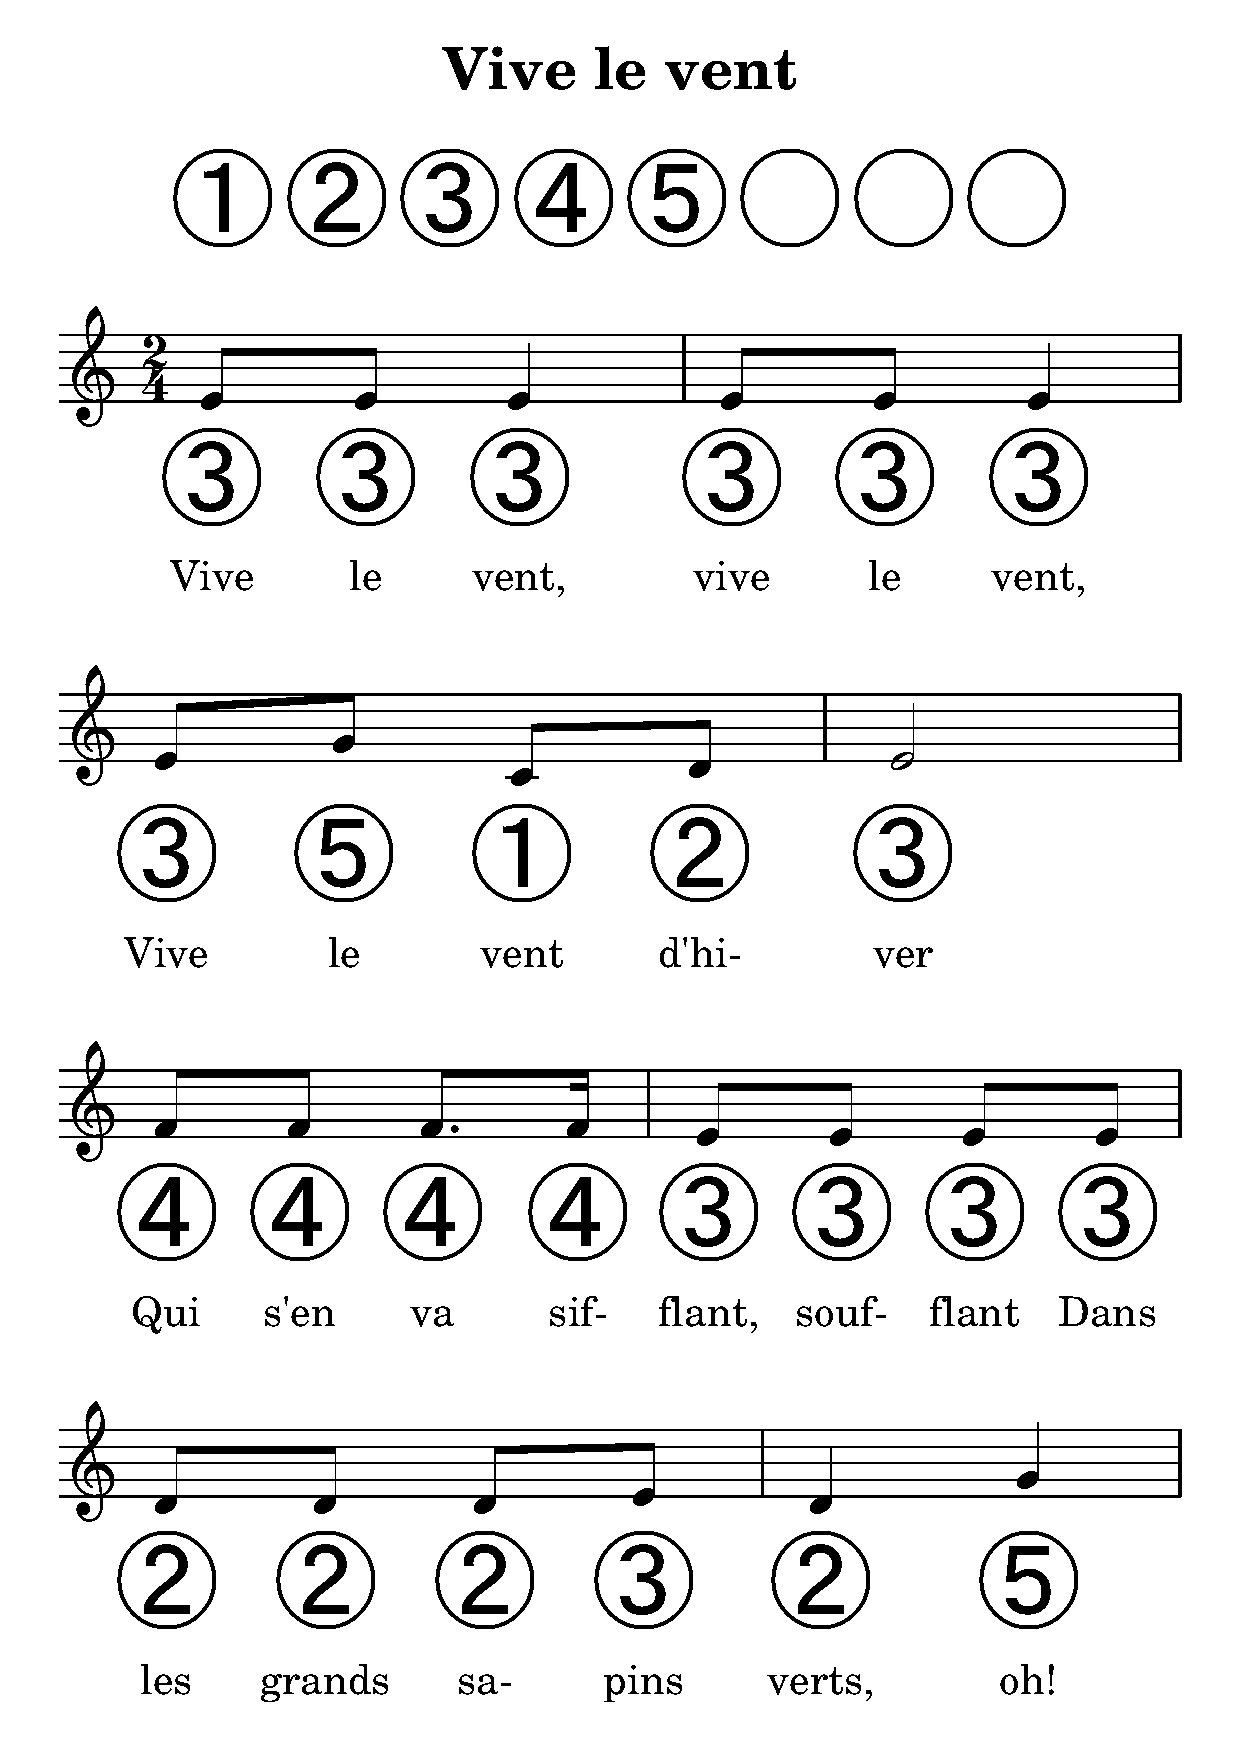
\includepdf[pages=1-,pagecommand={\null\clearpage}]{vive_le_vent.pdf}

\clearleftpage

\addcontentsline{toc}{section}{Frère Jacques}
\includepdf[pages=1-,pagecommand={\null\clearpage}]{frere_jacques.pdf}

\clearleftpage

\addcontentsline{toc}{section}{À la claire fontaine}
\includepdf[pages=1-,pagecommand={\null\clearpage}]{a_la_claire_fontaine.pdf}

\clearleftpage

\addcontentsline{toc}{section}{Le roi Dagobert}
\includepdf[pages=1-,pagecommand={\null\clearpage}]{dagobert.pdf}

\clearleftpage

\addcontentsline{toc}{section}{À la pêche aux moules}
\includepdf[pages=1-,pagecommand={\null\clearpage}]{a_la_peche_aux_moules.pdf}

\clearleftpage

\addcontentsline{toc}{section}{Bonjour, belle Rosinne}
\includepdf[pages=1-,pagecommand={\null\clearpage}]{rosinne.pdf}


\end{document}
